\documentclass[a4paper, 12pt]{report}

%====================== PACKAGES ======================

\usepackage[french]{babel}
\usepackage[utf8x]{inputenc}
%pour gérer les positionnement d'images
\usepackage{float}
\usepackage{amsmath}
\usepackage{graphicx}
\usepackage[colorinlistoftodos]{todonotes}
\usepackage{url}
%pour les informations sur un document compilé en PDF et les liens externes / internes
\usepackage{hyperref}
%pour la mise en page des tableaux
\usepackage{array}
\usepackage{tabularx}
%pour utiliser \floatbarrier
%\usepackage{placeins}
%\usepackage{floatrow}
%espacement entre les lignes
\usepackage{setspace}
%modifier la mise en page de l'abstract
\usepackage{abstract}
%police et mise en page (marges) du document
\usepackage[T1]{fontenc}
\usepackage[top=2cm, bottom=2cm, left=2cm, right=2cm]{geometry}
%Pour les galerie d'images
\usepackage{subfig}
% Pour les enumerations
%\frenchbsetup{StandardLists=true}
%\usepackage{enumitem}

% pour l'ecriture de code

\usepackage{listings}
\usepackage{color}

\definecolor{mygreen}{rgb}{0,0.6,0}
\definecolor{mygray}{rgb}{0.5,0.5,0.5}
\definecolor{mymauve}{rgb}{0.58,0,0.82}

\lstset{ %
  backgroundcolor=\color{white},   
  basicstyle=\footnotesize,        
  breakatwhitespace=false,         
  breaklines=true,                 
  captionpos=b,                    
  commentstyle=\color{mygreen},    
  deletekeywords={...},            
  escapeinside={\%*}{*)},          
  extendedchars=true,              
  frame=single,	                   
  keepspaces=true,                 
  keywordstyle=\color{blue},       
  language=Octave,                 
  morekeywords={*,...},            
  numbers=left,                    
  numbersep=5pt,                   
  numberstyle=\tiny\color{mygray}, 
  rulecolor=\color{black},         
  showspaces=false,                
  showstringspaces=false,          
  showtabs=false,                    
  stringstyle=\color{mymauve},     
  tabsize=2,	                   
  title=\lstname                   
}
%pour les formules
\usepackage{amsmath}
\frenchbsetup{StandardLists=true}
\usepackage{enumitem}
%====================== INFORMATION ET REGLES ======================

%rajouter les numérotation pour les \paragraphe et \subparagraphe
\setcounter{secnumdepth}{4}
\setcounter{tocdepth}{4}

\hypersetup{							% Information sur le document
pdfauthor = {Premier Auteur,
			Deuxième Auteur,
			Troisième Auteur,
    		Quatrième Auteur},			% Auteurs
pdftitle = {Nom du Projet -
			Sujet du Projet},			% Titre du document
pdfsubject = {Mémoire de Projet},		% Sujet
pdfkeywords = {Tag1, Tag2, Tag3, ...},	% Mots-clefs
pdfstartview={FitH}}					% ajuste la page à la largueur de l'écran
%pdfcreator = {MikTeX},% Logiciel qui a crée le document
%pdfproducer = {}} % Société avec produit le logiciel

%======================== DEBUT DU DOCUMENT ========================

\begin{document}

%régler l'espacement entre les lignes
\newcommand{\HRule}{\rule{\linewidth}{0.5mm}}

%page de garde
\begin{titlepage}
\begin{center}

% Upper part of the page. The '~' is needed because only works if a paragraph has started.

\includegraphics[width=0.35\textwidth]{./log_nanterre}~\\[1cm]

\textsc{\LARGE Université Paris Ouest Nanterre}\\[1.5cm]

\textsc{\Large }\\[0.5cm]

% Title
\HRule \\[0.4cm]

{\huge \bfseries Mémoire : \\
Optimisation d'attribution de primes ou de promotions au mérite  \\[0.4cm] }

\HRule \\[1.5cm]

% Author and supervisor
\begin{minipage}{0.4\textwidth}
\begin{flushleft} \large
\emph{Auteur:}\\
\textsc{Macylia LALMAS}\\
\end{flushleft}
\end{minipage}
\begin{minipage}{0.4\textwidth}
\begin{flushright} \large
\emph{Encardeur:} \\
Reda \textsc{BENDRAOU}\\
\end{flushright}
\end{minipage}

\vfill

% Bottom of the page
{\large 9 juin 2017}

\end{center}
\end{titlepage}

%page blanche
\newpage
~
%ne pas numéroter cette page
\thispagestyle{empty}
\newpage

\renewcommand{\abstractnamefont}{\normalfont\Large\bfseries}
%\renewcommand{\abstracttextfont}{\normalfont\Huge}

\begin{abstract}
\hskip7mm

\begin{spacing}{1.3}
    Le présent travail réalisé au cours de mon deuxième semestre d’études s'inscrit dans le cadre de l'obtention du Master 2 MIAGE. 

    L'objectif de ce mémoire est la recherche et production d'un modèle informatisé optimum relatif à la décision d'attribution des primes et/ou de promotions combinant les avantages de différentes méthodes et ce dans le cadre de la gestion des ressources humaines. C'est en testant les différentes méthodes relatives à cette fonction décisionnelle en recherchant l’élimination des aspects subjectifs du facteur humain lors de cette opération (tache de gestion primordiale pour le devenir  de l'entreprise).\\

\end{spacing}
\end{abstract}

\setcounter{tocdepth}{1}
\tableofcontents
\listoffigures
\thispagestyle{empty}
\setcounter{page}{0}
%ne pas numéroter le sommaire

\newpage

%espacement entre les lignes d'un tableau
\renewcommand{\arraystretch}{1.5}

%====================== INCLUSION DES PARTIES ======================

~
\thispagestyle{empty}
%recommencer la numérotation des pages à "1"
\setcounter{page}{0}
\newpage

\chapter*{Introduction}
\addcontentsline{toc}{chapter}{Introduction}

Le traitement du sujet faisant l'objet de cette étude a trait au domaine des ressources humaines dans le cadre du fonctionnement d'une entreprise où se côtoient différents groupes humains  et catégories de salariés dans diverses fonctions.\\
La gestion des ressources humaines a évolué et a développé des méthodes et des règles qui tiennent compte du contexte et des impératifs amenant à chaque fois les responsables à opter pour la méthode la plus appropriée tant au niveau organisationnel qu'en termes de coût pour en rentabiliser tous ses aspects.\\
Cette approche des décideurs est en réalité dictée par l'importance du contexte d'évolution de toute entreprise quelle que soit son activité et le degré d'impact de  chaque méthode d'évaluation de ces ressources humaines.\\

 
Aujourd'hui, les entreprises évoluent dans un environnement de plus en plus concurrentiel, changeant et complexe. En particulier, sur le marché de l'emploi où règne une concurrence exacerbée, l'exigence première est non seulement de recruter des ressources humaines de qualité, présentant un haut niveau de qualification, mais aussi de les fidéliser « réduire les comportements d'absentéisme et de démission » ainsi que de les motiver « des employés plus efficaces et plus appliqués ».\\
L'investissement sur les collaborateurs a un impact direct sur la satisfaction client, et réciproquement.\\
Le lien entre la satisfaction des employés et celle des clients est indiscutable. Des employés heureux ne signifient pas uniquement que ces employés ont le moral mais qu'ils seront plus efficaces et plus appliqués.\\ 
Selon une récente étude de Gallup, le désengagement des employés coûte plus de 300 milliards de \$US par an à l'industrie américaine. \\
Une autre étude montre que 72\% des employés motivés sont persuadés qu'ils peuvent influencer positivement le service clients. Cette étude visait à déterminer l'impact des employés motivés sur la satisfaction des clients :
\begin{itemize}
\item	Premièrement, le niveau d'engagement des employés a un impact sur la satisfaction des services fournis aux clients. A chaque augmentation de deux points de la motivation de l'employé, la satisfaction du client augmente d'un point.
\item	Deuxièmement, globalement environ 20\% des variations sur le score de satisfaction sont liées aux changements de scores des employés.\\
\end{itemize}

La motivation et satisfaction des employés sont fluctuantes et varient en fonction de très nombreux facteurs. En entreprise, il est question de bien-être et de volonté et pour que les salariés restent satisfaits et motivés, l’entreprise doit rester attentive à leurs besoins, au regard bien sûr de leur mérite\\
Ces besoins sont schématisés par la pyramide des besoins, une théorie élaborée à partir des observations réalisées dans les années 1940 par le psychologue Abraham Maslow sur la motivation. 

%inclusion d'une mage dans le document
\begin{figure}[!ht]
\begin{center}
%taille de l'image en largeur
%remplacer "width" par "height" pour régler la hauteur
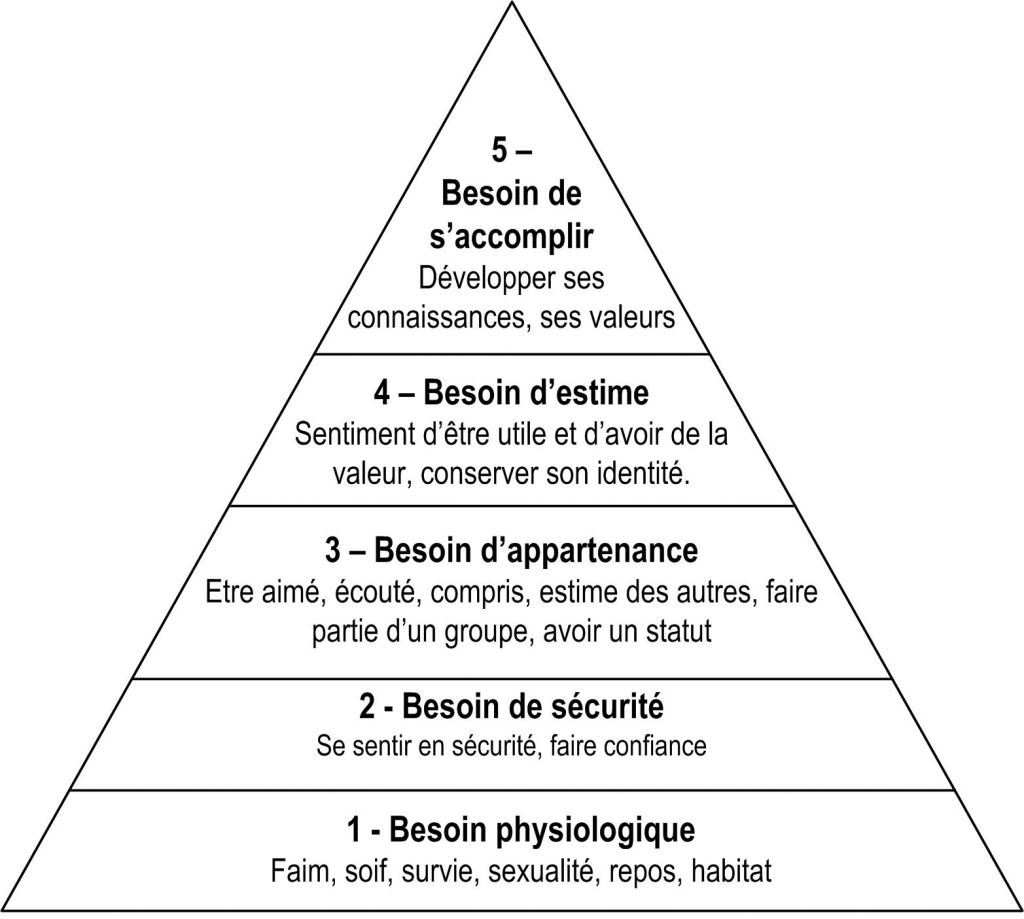
\includegraphics[width=9cm]{introduction/schema_introduction}
\end{center}
%légende de l'image
\caption{pyramide des besoins}
\end{figure}

\newpage

Voici quelques pistes utilisées par les entreprises aujourd’hui pour entretenir la motivation et satisfaction des salariés :
\begin{enumerate}
\item la motivation par le cadre de travail
\item la motivation par les avantages
\item la motivation par un voyage
\item La motivation par l’argent \\
\end{enumerate}

La promotion et/ou prime  peuvent être accordées en fonction des objectifs atteints par le salarié, ou en fonction du nombre d'années passées dans l'entreprise, une clause du contrat de travail prévoit fréquemment l'accord automatique de ces avancements, et suite à une simple demande de votre part, votre employeur appréciera alors vos résultats et vos compétences pouvant justifier une augmentation de vos responsabilités.\\
En plus de vos capacités techniques et intellectuelles, il peut être très avantageux de faire preuve de fiabilité et d'empathie.\\ Le contact relationnel avec les supérieurs et collègues peut s'avérer déterminant lorsqu'il s'agit d'arbitrer l'attribution d'une promotion.\\

Il existe 3 manières de promouvoir les employés :
\begin{enumerate}
\item Promouvoir les plus compétents
\item Promouvoir les moins compétents
\item Promouvoir au hasard
\end{enumerate}
\newpage
D’après le principe de Peter qui part du postulat que : «  tout employé compétent sera promu tôt ou tard à un poste qui surpasse ses compétences »,avec comme conséquence à terme d'avoir tous les postes occupés par des incompétents (situation inimaginable dans la pratique).
La solution qui est proposée pour un dirigeant constatant qu'il a des cadres supérieurs incompétents, c’est de recourir à la « sublimation percutante » consistant à accorder à une personne incompétente une promotion vers un poste plus prestigieux en apparence, mais en fait à responsabilité très inférieure, et pour les personnes constatant leur propre incompétence c’est de se maintenir à un poste auquel on est compétent.Ceci , non seulement dans l'intérêt de l'organisation où l'on travaille, mais aussi parce qu'être compétent à son poste est un facteur de bonheur personnel. Toutefois, Peter constate que le refus d'une promotion est mal vu par l'entourage des personnes..\\
Des chercheurs italiens ont réussi à prouver de manière scientifique que la meilleure manière d'attribuer les promotions c’était de les distribuer au hasard. Mais aussi rigoureuse soit-elle, cette expérience devrait ne servir à rien.\\
Pour faire cette recherche, ils sont partis de leur envie de contrer le "Principe de Peter", ils se sont lancés à la recherche d’un moyen de distribuer les promotions. Ils ont mis au point un simulateur qui compare les performances de l’entreprise selon trois scénarios. Dans le premier, la société promeut les employés les plus compétents. Dans le deuxième, elle choisit au contraire les moins compétents. Dans le dernier, elle nomme les managers au hasard. Et là, les chercheurs découvrent qu'avec la méthode aléatoire, la productivité augmente d’une dizaine de points! Alors qu’avec les deux autres scénarios, elle baisse, inévitablement.\\
 Observation: Les chercheurs soulignent néanmoins que la promotion au mérite n’est pas nécessairement plus juste. La mesure du mérite par un manager comporte une part de subjectivisme. Il reste que la promotion au hasard, même si son efficacité est prouvée, est indéfendable vis-à-vis des équipes. Et donc se pose la question de savoir comment motiver ses salariés si leur implication n’est pas récompensée?\\
Ce qui nous amène à mon travail car pour garder la motivation et en même temps avoir des résultats moins subjectifs , nous nous  proposons d’appliquer la méthode au mérite c’est-à-dire attribuer les promotions aux plus compétents en introduisant la solution informatisée en minimisant l’impact humain au maximum.\\   


\section*{Problématique}

L’un des coûts les plus élevé des entreprises est le roulement du personnel.  Un des plus grand défis est certainement de trouver le moyen de créer un environnement favorisant la mobilisation qui peut engendrer la productivité.\\
Non seulement, il est coûteux de procéder à des modifications d'organigramme (mouvement du personnel,mais les changements apportés affectent aussi le moral du reste du personnel. Afin de minimiser cela, l’entreprise doit s’employer à satisfaire et motiver ses salariés « primes, promotions, … », mais la répartition des promotions entre plusieurs individus exerçant la même fonction dans une même unité de production est un éternel sujet de discussions. Comment faut-il augmenter les salariés? Faut-il attribuer une promotion à tel salarié mais pas à l’autre ? Quelle prime donner à qui ? Et surtout comment attribuer ces primes de manière juste et équitable envers tous les employés ? Car la mesure du mérite par un manager comporte un aspect  subjectif.\\


\section*{Objectif}
Une solution qui peut paraître simple consiste à construire un outil d’aide à la décision pour le classement des salariés sur la base du mérite et de manière décroissante .Cela n’écartera toujours pas l’impact humain mais le minimisera car l’outil a pour but principal de guider les managers dans leurs décisions et de rassurer les employés par rapport à l’équité de la décision.\\
 \\
L’objectif de mon projet est de concevoir un outil d’aide à la décision pour apporter des réponses pertinentes à la problématique d’attribution de promotion ou de prime et cela en testant différentes méthodes d’évaluation des salariés d’une entreprise.  


\newpage






\chapter{Les différentes méthodes d’attribution de primes et de  promotions existantes}


\section{Introduction}

Généralement dans les entreprises, c’est au cours des réunions annuelles que sont fixées les primes et augmentations de salaires et où chaque responsable d’unité défend les intérêts de ses salariés pour obtenir la meilleure part possible de l’enveloppe salariale de l’entreprise. \\
C’est ainsi qu’autour de la table de réunion, sous l’autorité du directeur du personnel qui fera l’arbitrage, on discute sur des notes et des appréciations faites dans le meilleur des cas avec les mêmes barèmes, mais données par des chefs différents, plus ou moins bienveillants.\\ 
En clair, l’augmentation « promotion » de chaque salarié dépend de ce que son chef dira ou montrera le jour de la réunion le concernant. Et plus l’entreprise est grande plus ce fléau empire.\\
Aujourd’hui, pour moderniser cela et pour une amélioration du rendu des employés, plusieurs méthodes ont vu le jour « le ranking, Le management par objectifs (MBO) … »
\\
\section{Le ranking}
\subsection{Qu'est-ce que le " ranking " ?}

Le ranking, est une pratique managériale qui tend à évaluer puis classer les collaborateurs afin d'éliminer les moins performants, cette technique de notation, qui a vu le jour voilà quelques années déjà, est surtout appliquée dans les pays anglo-saxons.\\ 
En clair, elle consiste à classer les salariés, en fonction de leur performance individuelle, selon une distribution fixée à l’avance (20\% très performants, 10\% peu performants, 70\% efficaces)..\\ 
Le choix de cette distribution s’appuie sur une loi statistique représentée par une courbe de Gauss. Les principes sont simples. Le premier est de ne pas cantonner les évaluations par direction, mais au contraire d’utiliser le levier de la transversalité inter-directions.\\ En somme, ce sont des comités constitués des responsables de chaque direction qui vont évaluer l’ensemble des collaborateurs.
\newpage
\subsection{Les différentes étapes du ranking }
Schématiquement, cela fonctionne en quatre étapes : 
\begin{itemize}
\item Premièrement, la DRH répartit les collaborateurs à évaluer en plusieurs groupes sur la base du poids de leur poste et non selon le titre de la fonction du collaborateur.
\item En second lieu, chaque responsable doit réaliser un entretien avec le collaborateur afin de définir les succès de l’année et ses échecs …
\item La réunion d’évaluation, troisième étape, a pour objectif ultime de classer les membres d’un groupe de collaborateurs de poids de postes comparables par ordre décroissant. Pour ce faire, chaque responsable devra mettre en avant des arguments valables pour placer ses collaborateurs ou ceux des autres, dans les premières places et ainsi de suite jusqu’aux dernières places.
\item Enfin, pour être validé, chaque classement requiert le quorum de l’ensemble des responsables.
\end{itemize}

\subsection{Les avantages et inconvénients du ranking}
Cette méthode présente plusieurs avantages :
\begin{itemize}
\item Elle permet de faire évaluer un collaborateur par d’autres responsables ce qui leur permet de connaître ses performances et facilite la mobilité interne.
\item De plus, les décisions prises requièrent le quorum de l’ensemble des responsables, et lorsqu’elles sont bonnes, elles sont plus flatteuses que celles prises par un seul responsable. Et au contraire, une évaluation moyenne, ou mauvaise, est toujours, plus facile à annoncer, pour un manager lorsqu’il se cache derrière une décision de groupe.
\item Ce genre de réunion permet à chaque responsable de défendre les places de leurs protégés dans les meilleures positions du ranking, en exposant des résultats concrets, qui valent mieux que des croix sur des critères dans le système de notation classique. Il devra lutter contre les arguments et contre-arguments des autres responsables qui recherchent aussi à prendre les premières places.
\item Il y a un budget dédié aux performants et pas de budget dédié par direction et c’est une sacrée différence pour la fiche de paie des personnes sélectionnées comme performants ! Cela permet de rejoindre l’objectif fixé par tout système de notation : attirer, retenir et encourager les plus performants.
\end{itemize}

L’inconvénient majeur de cette méthode c’est que la mise en œuvre d'un mode d'évaluation reposant sur un classement des salariés en catégories en fonction de quotas impératifs fixés à l'avance est illicite.\\

D'ailleurs,quelques tribunaux se sont déjà prononcés sur la licéité de ce procédé au vu de  certaines firmes dont l'augmentation ininterrompue des performances est imposée comme   règle et le ranking  devenant l'instrument de mesure privilégié.

\section{Le management par objectifs (MBO)}
\subsection{Le management par objectifs (MBO)}
Le management par objectifs est une pratique très courante dans les entreprises actuelles, c’est le liant entre l'atteinte des objectifs et donc les résultats, d'une part, et le développement de l'individu et son implication, d'autre part.\\
Le système de management par objectifs « Managment by objectives »« MBO » a été proposé en 1954 par Peter Drucker.\\ 
Il présuppose que les mentalités changent et que les individus ne considèrent plus qu’ils sont là pour exécuter une somme de tâches, mais qu’ils sont là pour atteindre l’objectif de leur poste de travail.\\ 
Il anticipe en cela la théorie de la motivation de Frederick Hertzberg qui établit, en 1959, que pour être motivé au travail, l’être humain a besoin de connaître le rôle de son poste dans la marche de l’entreprise et d’assumer la responsabilité des résultats qu’il doit obtenir.

\subsection{Les différentes étapes du MBO}
Le procédé s’effectue de manière annuelle :
\begin{enumerate}
\item Chaque membre du personnel rencontre son responsable en entretien annuel.
\item Ensemble, ils déclinent l’objectif général du poste en sous objectifs mesurables, réalistes, inscrits dans la durée et classés par ordre de priorité. Chaque objectif doit être doté des moyens nécessaires à son accomplissement.
\item Ils se séparent après accord sur le résultat à atteindre et les indicateurs de réussite( un compte rendu d’entretien entérine cet accord).
\item Le collaborateur exécute son travail en restant maître de ses méthodes. Le cas échéant, il décline ses propres objectifs en objectifs pour ses collaborateurs.
\item Responsable et collaborateur se rencontrent régulièrement pour faire le point, à des dates qu’ils ont préalablement arrêtées. Le responsable apporte son aide en savoir, en expérience, en facilitation, en rectification … Mais l’objectif ne change pas. Seuls sont traités les moyens de franchir les obstacles.
\item Lors de l’entretien annuel suivant, responsable et collaborateur se retrouvent pour mesurer le pourcentage de réalisation des objectifs annuels.
\item Ils décident d’actions susceptibles de corriger l’écart entre l’objectif et le résultat. ça peut-être une adaptation de l’objectif, une modification des moyens, une formation pour le collaborateur ou son équipe, etc.
\item Ils optimisent ainsi chaque objectif, en ajoutent si la situation l’exige, annulent ceux qui n’ont plus lieu d’être (projet achevé ou annulé).

\end{enumerate}

\subsection{Les avantages et inconvénients du MBO}

L’avantage principal de cette démarche du management par objectifs mise avant tout sur une relation gagnant-gagnant entre l'employeur et le collaborateur « collaborateur motivé et employeur  satisfait ».\\
L’inconvénient de cette méthode c’est que l’évaluation des salariés se fait sur la base d’un seul critère  « l’atteinte ou pas de l’objectif fixé ».


\section{Le management en équipe}
\subsection{Qu'est-ce que le management en équipe}
Le management en équipe consiste à évaluer les capacités des salariés en fonction de critères objectifs, indépendants des variations aléatoires des performances personnels.\\
Le principe est de considérer l’entreprise comme un système dont les salariés sont des éléments interdépendants c’est-à-dire on ne mets plus l’accent sur des résultats individuels de chaque salarié, mais plutôt sur les résultats commun à tous les salariés.\\
Shewhart, un grand statisticien, chercheur au département qualité de AT\&T, a mis au point en 1939 une méthode pour étudier et améliorer le processus de toute activité de production de biens ou de services, en identifiant des événements significatifs parmi un grand nombre d'événements qui ne le sont pas. Et cela en appliquant le calcul des probabilités à ce type de processus. Le but de cette approche est de supprimer le gâchis matériel et humain du management ordinaire.\\ 
Ce type de management oblige à traiter l’ensemble des processus de production comme un système organique où il est contre-productif de faire appel à la concurrence entre les fournisseurs de l’entreprise, les départements, les employés, etc. Cette conception s'oppose radicalement à la théorie enseignée dans les business schools et aux pratiques dominantes. 

\subsection{La pratique de la méthode du management en équipe}

Bien qu’une telle procédure ne soit pas imposée par la loi, il est important que les directeurs et les chefs de service s’entretiennent en tête à tête avec leurs subordonnés au moins une fois par an pour faire le bilan de leurs activités. \\
L’entreprise aurait une procédure d’évaluation annuelle et contrairement aux autres méthodes  La grille d’évaluation ne comportera pas de notes de performances, ou en d’autres termes pas de bilan individuel résultats / objectifs comme dans le MBO mais elle comportera plutôt des notes relatives aux aptitudes professionnelles, aux compétences dans le métier et au degré de participation de chaque salarié à l’amélioration globale de l’entreprise. \\
Ainsi,organiser des groupes de travail consacrés à des projets d’amélioration des processus où les salariés sont invités à y prendre part, cela fournira un bon moyen d’évaluer leur degré de participation.\\
Cette méthode permet d’identifier les salariés « hors contrôle » qui représentent généralement, on le sait, moins de 10\% dans chaque catégorie. Par définition, ce sont ceux dont les aptitudes sont en dehors de l’intervalle de contrôle du processus. Il faut donc chercher les causes de ces variations. Quand une aptitude est supérieure à l’intervalle, une étude avec l’intéressé peut conduire à une amélioration du processus. Quand elle est inférieure, une étude permet de découvrir quel est le handicap de l’intéressé.\\ 
Par exemple dans une petite entreprise, un graphique de contrôle avait montré que l’aptitude d’un magasinier était inférieure à l’intervalle de contrôle. L’étude a révélé qu’il avait besoin de lunettes : le problème a été vite réglé. Cette étude peut se faire à l’aide d’outils d’analyse statistique à l’usage des non statisticiens que l’on trouve sur Internet.\\ 
Quand un salarié est hors contrôle vers le haut, il pourra faire l’objet d’une promotion. Celui qui est hors contrôle vers le bas a besoin d’aide, peut-être d’une formation. Si l’écart persiste malgré l’aide qui lui est donnée, il faudra lui  changer de poste ou le licencier.
\newpage
\subsection{Les avantages et inconvénients du management en équipe}
L’avantage de cette méthode c’est qu’elle privilégie la coopération à la compétition et utilise  des moyens rationnels pour réussir économiquement ce qui incite les salariés à travailler en équipe pour atteindre des objectifs communs.\\
Un autre avantage c’est le fait qu’elle permet de ne pas imputer injustement aux acteurs les défaillances de la production, mais de les imputer au système où ils interviennent.\\ 
L’inconvénient de cette méthode c’est que l’absence d’objectif et  de concurrence  peut engendrer une diminution de la motivation de chaque employé à donner le meilleur de lui-même en comptant sur le travail des autres.

\section{conclusion}
Chacune des méthodes d’évaluation citée dans ce chapitre, présente des points positifs et des points négatifs, ce qui m’amène à proposer une solution plus au moins hybride afin d’améliorer ces points négatifs et essayer de préserver les points positifs de ces solutions.\\
Ci-dessous ,nous présenterons la configuration du contexte dans lequel  s'intégrera  la solution proposée.     
 


\chapter{L’aide multicritère à la décision }

\section{Introduction}

Les outils d'aide à la décision permettent d'apporter des réponses pertinentes à des problématiques diverses mettant en œuvre plusieurs choix possibles (implantation de sites industriels, stratégie de dépollution d'un lac, constitution de portefeuilles de valeurs, etc.), d'aider au diagnostic et, plus généralement, de faciliter la prise de décision stratégique ou opérationnelle en environnement imprécis et/ou incertain.\\
La détermination de la « meilleure » action (optimale, de meilleur compromis...) constitue un défi intellectuel perpétuel en sciences et en génie. L’aide multicritère à la décision s’est alors développée pour offrir à la fois une démarche et des outils de solutions à des problèmes décisionnels complexes d’après KEENEY R L. Ainsi, l’analyse multicritère est aujourd’hui considérée comme l’une des branches les plus importantes de la recherche opérationnelle et des théories de la décision.\\
Dans notre cas l’outil d’aide à la décision développé devra aider à la sélection des employés les plus méritants à acquérir une promotion ou prime …  et cela grâce à des méthodes mathématiques d'analyse multicritère qui fournissent un classement des employés.

\section{Définition de l’aide à la décision}
De manière générale l’aide à la décision est l’activité de celui qui, prenant appui sur des modèles clairement explicités mais non nécessairement complètement formalisés, aide à obtenir des éléments de réponses aux questions que se pose un intervenant dans un processus de décision, éléments concourant à éclairer la décision.\\
Elle est généralement sollicitée par des organisations dans le cas où elles sont confrontées à des problèmes complexes, par exemple, de planification, d’allocation et de gestion de ressources, de choix et d’évaluation, etc. Ces problèmes induisent une décision (ou une série de décisions) lourde(s) de conséquences, et que l’expérience et le bon sens, seuls, ne suffisent pas à éclairer. Cette série de décisions s’inscrit dans un processus appelé « processus de décision ».\\
Dans la littérature, il est défini par A. Tsoukiàs comme étant « un espace d’interaction, pouvant évoluer dans l’espace et dans le temps, dans lequel tous les intervenants partagent des préoccupations qui sont parfois contradictoires (améliorer l’approvisionnement, diminuer les coûts) ». L’existence d’un tel espace est justifiée par la présence d’un objectif (préoccupation) final.\\ 
Le fait que le processus de décision soit évolutif, nous laisse supposer que la préoccupation finale peut l’être également. L’aide à la décision, sollicitée par les intervenants dans ce processus, doit aider à répondre, souvent indirectement, à cette préoccupation finale.\\ 
\newpage
L’aide à la décision n’aide pas, nécessairement, à répondre directement à la préoccupation finale mais peut se limiter à certaines questions traduisant les préoccupations de certains intervenants.\\ 
Cependant, nous pensons qu’il est important de s’assurer, en répondant à ces préoccupations, que nous apportons aussi des éléments de réponses à la préoccupation finale et que l’aide à la décision soit cohérente avec l’évolution de cette préoccupation

\section{La problématique de la décision}
La problématique de décision peut être perçue comme étant une orientation de l’investigation qu’on adopte pour un problème de décision donné. Elle exprime les termes dans lesquels le décideur pose le problème et traduit le type de la prescription qu’il souhaite obtenir. Nous pouvons distinguer quatre problématiques en aide multicritère à la décision:
\begin{itemize}
\item Problématique de choix (P.$\alpha$)
\\Elle consiste à sélectionner un sous ensemble aussi restreint que possible de l’ensemble des actions A "une action représente l’objet de la décision", contenant les meilleures actions. L’idéal est d’obtenir une seule et meilleure action. Mais à cause de la nature conflictuelle des critères, il est préférable de fournir au décideur quelques actions qui représentent différentes variantes de la "meilleure action". Évidemment, le résultat final peut être raffiné en utilisant de l’information additionnelle ou avec une analyse plus approfondie. 
\begin{figure}[!h]
\begin{center}
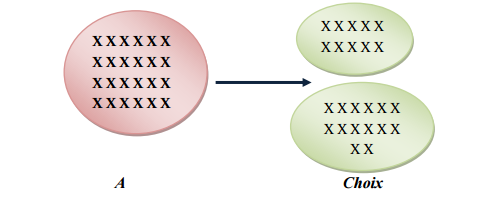
\includegraphics{aide_multicrit_decision/prob_de_choix.png}
\end{center}
\caption{Problématique de choix}
\end{figure}
\item Problématique de tri (P.$\beta$): 
\\Elle consiste à affecter chaque action à un ensemble de catégories prédéfinies. Cette formulation est adéquate lorsque le problème de décision consiste à examiner chaque action indépendamment des autres (en tenant compte que des caractéristiques intrinsèques de chaque action) dans le but de proposer une recommandation parmi un ensemble des recommandations spécifiées en avance. Chaque recommandation peut être associée avec une catégorie. Le problème de décision est alors vu comme trier les actions potentielles aux différentes catégories définies en termes de normes prédéfinies. La procédure de tri doit être définie de telle sorte que chaque action est affectée à une et seule catégorie. Formellement, une prescription consiste à une partition de A.
\begin{figure}[!h]
\begin{center}
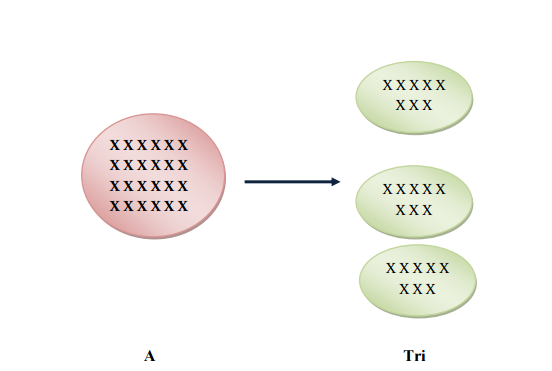
\includegraphics{aide_multicrit_decision/prob_de_tri.png}
\end{center}
\caption{Problématique de tri}
\end{figure}
\newpage
\item Problématique de rangement (P.$\gamma$): 
\\Elle consiste à ranger les différentes actions en allant de la meilleure action à la moins bonne. Cette problématique est intéressante lorsque les actions sont à différencier selon leur intérêt relatif. L’idéal est d’obtenir un ordre complet. Cependant, à cause de la nature conflictuelle des critères, à l’imprécision, à l’existence de systèmes de valeurs différents, il est souvent plus réaliste de présenter au décideur un ordre partiel. Il est à noter qu’en pratique, le rangement peut être nécessaire seulement pour les actions les plus intéressantes. Formellement, la prescription est un ordre partiel, une relation transitive définie sur A (ou un sous ensemble de A).
\begin{figure}[!h]
\begin{center}
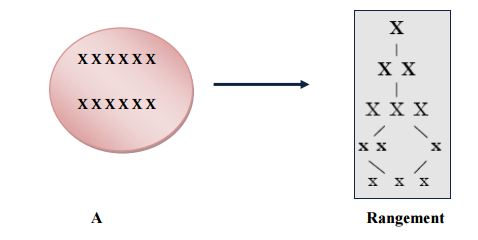
\includegraphics{aide_multicrit_decision/prob_de_rangement.png}
\end{center}
\caption{Problématique de rangement}
\end{figure}
\newpage
\item Problématique de description (P.$\delta$): 
 \\Elle consiste simplement à décrire les actions et leurs conséquences et non pas à les comparer comme c’est le cas avec les trois autres problématiques précédentes. Ici, il n’existe pas une prescription et la procédure d’investigation est cognitive.


\begin{figure}[!h]
\begin{center}
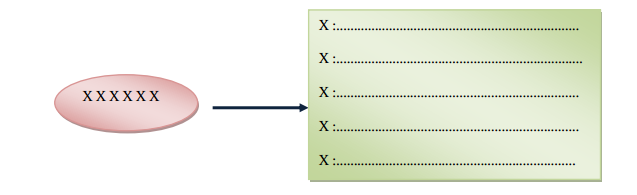
\includegraphics{aide_multicrit_decision/prob_de_descr.png}
\end{center}
\caption{Problématique de description}
\end{figure}
\end{itemize}

Le tableau récapitulatif des quatre problématiques en aide multicritère à la décision d’après B ROY.

\begin{figure}[!h]
\begin{center}
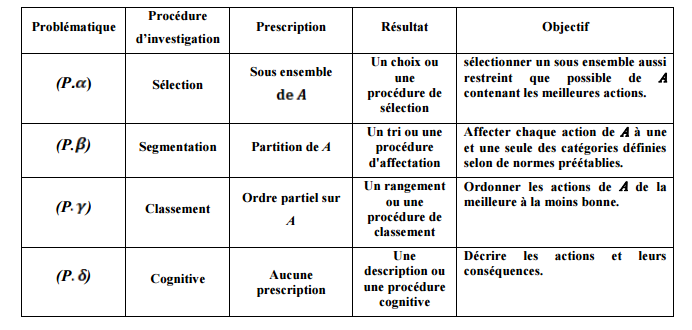
\includegraphics{aide_multicrit_decision/tabl_recap.png}
\end{center}
\caption{Tableau récapitulatif des quatre problématiques}
\end{figure}

Dans notre cas la problématique de mon travail c’est une problématique de rangement, car le but étant de faire un classement des salariés d’une entreprise d’après certains critères.

\newpage
\section{Le processus de décision}
Le processus de décision c’est l’enchaînement des trois phases suivantes d’après SIMON HA: 
\begin{itemize}
\item Phase de compréhension: analyse de la situation et du problème  
\item Phase de modélisation: formulation du problème (mise en évidence des écarts entre la situation actuelle et la situation objectée) et description des solutions potentielles 
\item Phase de sélection: choix d’une solution en fonction de critères concrets (objectifs, normes,…) ou abstraits (intuition, motivation,...), appréhendés par le décideur avec ou sans le soutien d’outils et de techniques d’aide à la décision
\end{itemize}
	
\begin{figure}[!h]
\begin{center}
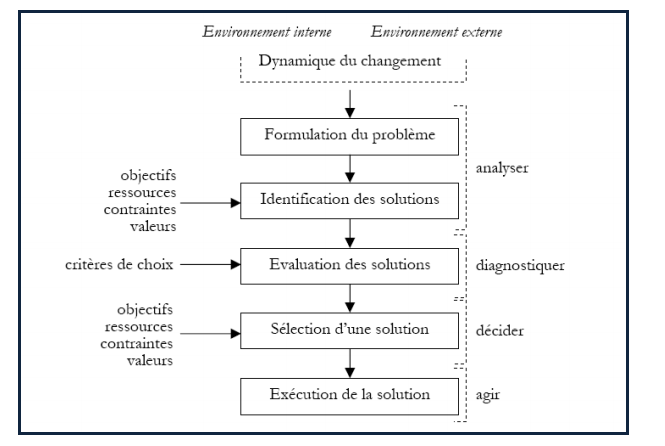
\includegraphics[height=6cm]{aide_multicrit_decision/environement.png}
\end{center}
\caption{Processus de décision}
\end{figure}

\section{Démarche de modélisation}
Dans cette section, nous allons nous intéresser aux types de modèles existants en aide à la décision et plus généralement aux approches fondées sur ces modèles. Il existe plusieurs types de modèles avec leur approche en aide à la décision :
\begin{itemize}
\item Approche normative\\
 Le décideur est rarement sollicité pour la construction de tels modèles. La validité des résultats fournis par le modèle repose sur leur cohérence avec les axiomes de la rationalité économique. Par exemple, on cherche un modèle permettant d’ordonner (du meilleur au moins bon) des investissements selon leur rentabilité économique. Si un investissement a est plus rentable qu’un investissement b et l’investissement b plus rentable qu’un investissement c, alors l’investissement a doit être plus rentable que l’investissement c.
\item Approche descriptive \\
Dans cette approche le décideur n’est également pas directement sollicité pour la mise en œuvre de ces modèles. Ces derniers sont généralement fondés sur des données ou des comportements existants (observations). Ils servent à décrire des phénomènes déjà réalisés pouvant se reproduire dans les mêmes conditions. La validité des résultats fournis par ces modèles repose sur l’observation d’autres phénomènes de même nature.
\item Approche prescriptive \\
L’approche prescriptive se différencie des deux premières par le fait qu’elle ne repose sur aucune information existante (rationalité économique ou observations). L’analyste doit collecter et structurer ces informations afin de construire un modèle. L’intervention du décideur n’est donc pas nécessaire lors de la construction du modèle, néanmoins, il intervient pour sa validation. Par exemple un médecin qui questionne un malade (pouvant décrire correctement ses symptômes mais ne sait pas ce qu’il a) afin de lui prescrire un traitement.
\item Approche constructive \\
La particularité de cette approche est que le décideur est sollicité, à la fois, lors de la construction du modèle mais aussi lors de sa validation. Les modèles sont donc fondés sur les connaissances des décideurs. L’homme d’étude cherche à les expliciter ou à les formaliser. La validation de ces modèles s’effectue, à l’image de l’approche prescriptive, par le décideur. Par exemple, lorsque l’homme d’étude cherche à construire un modèle représentant les préférences d’un décideur.

\end{itemize}

Parmi toutes ces approches, la dernière approche « Approche constructive » est la plus adéquate au travail que je veux effectuer, cela sera explicité en détail dans le chapitre suivant.

\section{Les méthodes multicritères d’aide à la décision}
Le recours aux méthodes multicritères d’aide à la décision s’est largement répandu depuis quelques années. Ces méthodes ont pour but la résolution des problèmes d'Aide à la décision multicritère. \\Elles constituent une étape importante du processus de décision, qui suit celle d'identification et de définition du problème, et aboutissent au choix d'une ou plusieurs solutions optimale(s).\\
Elles permettent également de répondre aux problématiques de tri et de rangement, par l'intermédiaire d'une procédure d'affectation et de classement respectivement.\\
Il existe trois grandes familles de méthodes multicritères. \\La première représente les méthodes utilisant un critère unique de synthèse « Agrégation a priori de critères en un critère unique » dont le principe consiste à agréger les performances d’une alternative en un seul critère. \\La deuxième famille représente les méthodes de sur-classement «Approche fondée sur le sur-classement» dont le principe consiste à comparer les alternatives par paires et enfin les méthodes interactives.\\ 
Nous allons présenter dans cette section les deux premières familles de méthodes, mais tout d’abord introduire quelques définitions importantes a la compréhension de ce qui suit.
\\
Actions, poids et critères de la décision\\
L’action représente l’objet de la décision et afin de différencier les actions réalisables de celles qui ne le sont pas, B. Roy nomme action potentielle ou alternative une action réalisable, c.-à-d. une action dont la mise en œuvre en pratique est envisageable. En aide multicritère à la décision l’ensemble des alternatives A est généralement construit sous forme d’une liste : A = {a1, a2, ...}.\\
Tandis que, un critère g est un outil permettant d’évaluer et de comparer des alternatives « actions » sur un point de vue bien défini. On note g(a) la performance de a sur le critère g, elle représente en général un nombre réel qui prend ses valeurs dans Xg (l’ensemble des valeurs possibles de g) défini explicitement.\\
Le poids quant à lui « w » c’est la valeur qui permet de mesurer l'importance d'un critère par rapport aux autres du point de vue du décideur.\\

\subsection{Agrégation a priori de critères en un critère unique}
Les préférences du décideur sont ramenées à un critère. Facile du point de vue mathématique mais les critères sont amalgamés dans la fonction de réponse. Une solution est présentée comme la meilleure, les actions sont complètement rangées\\
Cette approche englobe plusieurs méthodes « Somme pondérée, Analyse multicritère hiérarchique (AMCH) … »\\
Dans le cadre de mon travail j’ai choisis la somme pondérée et cela pour ça simplicité en terme de modélisation, son efficacité et son accessibilité mathématique.\\


\subsubsection{Somme pondérée}


\setcounter{secnumdepth}{4}


\paragraph{Présentation}
La méthode somme pondérée vise à construire un critère unique g agrégeant les P critères g1, g2, … gP et l’évaluation d’une action a $\epsilon$ A.

\paragraph{Données de départ}
La méthode somme pondérée a besoin de fixer les données de départ suivants :  
\begin{itemize}
\item m actions A1, A2, A3...Am
\item n critères C1, C2, C3...Cn
\item n poids correspondant chacun a un critère, un vecteur poids (W1, W2,...Wn) avec Wj > 0
\item aij = Uj(Ai), fonction d'utilité cardinale quotient, c'est-à-dire que cette fonction représente les écarts en plus de respecter l'ordre et pour laquelle il existe un zéro véritable. Ces données représentent les performances de chaque action sur chacun des critères.
\end{itemize}

\paragraph{Transformation des données}
\begin{enumerate}
\item Normalisation de tous les aij afin de conserver la proportionnalité entre les valeurs.
\item Normalisation des poids (la somme des poids = 1).
\item Mise en œuvre de la méthode Somme pondérée. 
Donc un critère unique pour toute action i
 
\begin{align*}
R(a_{i}) = \sum_{j=1}^{n}w_{j}a_{ij}
\end{align*}
\end{enumerate}
	

\paragraph{Les avantages et inconvénients de cette méthode}
La méthode de la somme pondérée possède trois avantages principaux :
\begin{enumerate}
\item Son modèle est largement utilisé grâce à sa simplicité 
\item La solution optimale d'une somme pondérée est efficace
\item pour de nombreux problèmes (combinatoires) ne modifie pas la complexité du problème  sous-jacent
\end{enumerate}
\newpage
Mais de nombreuses limites existent vis-à-vis de cette méthode:
\begin{enumerate}
\item La logique d’agrégation sous-jacente est totalement compensatoire, on préfère souvent utiliser des mécanismes d’agrégation partiellement compensatoires.
\item Pas de correspondance intuitive entre les valeurs des poids et la solution optimale proposée par somme pondérée.
\item L’interprétation des poids n’est pas très claire car ils intègrent à la fois :
\begin{itemize}
\item la notion d’importance relative des critères. 
\item un facteur de normalisation des échelles des critères. 
\end{itemize}
\end{enumerate}

La méthode de la somme pondérée nécessite donc d'avoir des critères comparables et d'intégrer l'influence de la normalisation préalable.



\subsection{Approche fondée sur le sur-classement}
Les préférences du décideur sont mathématiquement plus complexe mais correspondent mieux au problème. Solution du meilleur compromis, classements, cotations, ... Les problèmes de cette méthode sont de déterminer un sous-ensemble d'actions les meilleures (choix), de partitionner les actions en sous-ensemble spécifique (sélection), et de ranger les actions de la meilleure à la moins bonne (rangement).


\begin{figure}[!h]
\begin{center}
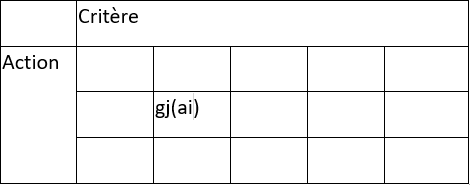
\includegraphics{aide_multicrit_decision/approche_surclassement.png}
\end{center}
\caption{approche de sur-classement}
\end{figure}

Cette approche englobe plusieurs méthodes « ELECTRE, PROMETHEE, ORESTE, MELCHIOR, TACTIC, ...»

Elles sont généralement utilisées quand :

\begin{itemize}
\item un critère au moins n’est pas quantitatif
\item les unités des critères sont très hétérogènes et leur codage en une échelle commune est difficile ou artificielle
\item la compensation entre avantages et désavantages sur différents critères n’est pas justifiable
\item des seuils de préférences ou de veto doivent être pris en compte.
\end{itemize}

Dans le cadre de ce travail, j’ai choisi d’utiliser une méthode de sur-classement car dans un processus d’aide à la décision, lors de la construction du modèle d’évaluation, il est rare d’aboutir uniquement à un seul critère correspondant à un point de vue unique sur lequel  le décideur exprimera ses préférences.\\ 
Il est donc nécessaire de considérer plusieurs points de vue dans la suite de la construction du modèle d’évaluation. Et parmi toutes les méthodes de sur-classement, j’ai choisi ELECTRE III car en plus de ses nombreux avantages que je citerai par la suite, la problématique de mon travail est comme spécifié précédemment une problématique de rangement et la méthode d’aide à la décision de sur-classement la plus appropriée à cette problématique est:l' ELECTRE III.

\subsubsection{La méthode ELECTRE}
La méthode d’analyse multicritère ELECTRE III est fondée sur la construction d’un classement d’alternatives, par le biais d’une approche d’agrégation partielle des performances. Cette méthode est ici appliquée à la gestion des promotions et primes pour les salariés.

\paragraph{Présentation}
ELECTRE signifie élimination et choix traduisant la réalité; c’est une famille de méthodes d'analyse multicritères développée en Europe à la fin des années 1960.\\
ELECTRE est une méthode non compensatoire d'aide à la décision multicritère introduite par Bernard Roy dans le but de Pallier les inconvénients de la somme pondérée.\\
Il existe plusieurs évolutions de cette méthode de surclassement « ELECTRE I, ELECTRE II, ELECTRE III … »\\
La méthode ELECTRE I a été élaborée par Bernard Roy en 1968. Avec l'aide de Patrice Bertier, il a ensuite développé la méthode ELECTRE II (B. Roy, P. Bertier 1971).\\
Les méthodes ELECTRE I et II ont été suivies de beaucoup d'autres parmi lesquelles :
\begin{itemize}
\item ELECTRE III (1978) qui utilise une relation de surclassement valuée et une procédure d'exploitation du graphe valué utilisant des techniques proches de celles de manipulation des nombres flous pour modéliser les pseudo-critères, utilisée généralement dans un besoin de classement.
\item ELECTRE IV (1982) est très simple et suppose que tous les critères (en fait des pseudo-critères) sont de même importance. Elle comporte deux relations de surclassement comme ELECTRE II mais un seul jeu de seuils de veto et la notion de concordance est traduite par une notion de majorité de critères en l'absence de toute pondération.
\item MELCHIOR (JP Leclercq 1984) est une méthode proche de ELECTRE II mais purement ordinale : elle utilise des pseudo-critères et utilise une relation d'ordre au lieu de poids pour refléter l'importance relative des critères. ELECTRE IV apparaît comme un cas particulier de MELCHIOR lorsque la relation d'ordre sur les critères est une équivalence.
Celle qui nous intéresse aujourd’hui et qui est la plus approprié à notre modèle d’aide à la décision :c’est ELECTRE III\\

\end{itemize}


\paragraph{Principe de la méthode Electre III}
La méthode Electre-III est une méthode d’analyse multicritère qui permet de résoudre des problèmes de classement, la méthode s’appuie sur la définition d’une relation de sur-classement S permettant de comparer deux actions a et b distinctes. En considérant un ensemble d’actions A= {a1, a2, a3,…,am}, il s’agit de classer les actions en les comparants par pairs. Chaque action est donc comparée aux autres sur la base des critères considérés. L’évaluation des actions est effectuée par une fonction réelle, pour chaque critère on définit l’ensemble des pseudo-critères G={g1,g2,…,gn} contenant l’évaluation de l’action sur l’ensemble des critères, une fonction a valeur réelle ((gj  : A → R).
La relation de sur-classement est noté (aSb) a surclasse b et elle est valide si les arguments d’un décideur d en faveur de la proposition ”a est au moins aussi bon que b” sont suffisamment forts, les arguments en faveur de aSb sont basés sur:
\begin{itemize}
\item Les évaluations de a (g1(a), g2(a), . . . , gp(a)) et de b (g1(b), g2(b), . . . , gp(b))
\item Une information sur les préférences de d (poids, seuils).
\end{itemize}
Sachant que si aucun argument ne peut être trouvé en faveur de aSb ni de bSa	on a l’incomparabilité.
\begin{itemize}
\item aSb et non bSa ⇒aPb (préférence)	
\item non aSb et bSa ⇒ bPa (préférence)
\item aSb et bSa ⇒ aIb (indifférence)
\item non aSb et non bSa ⇒ aQb (incomparabilité)
\end{itemize}

L’importance des critères dans la prise de décision est évaluée par un ensemble de poids W={W1,W2,…,Wn}. Pour cette méthode, les seuils d’indifférence, de préférence et de veto sont fonction de l’évaluation de l’action pour chaque critère. Pour une action a, évaluée par gj(a) pour le critère j, dans ce cas le seuil d’indifférence est noté qj(gj(a)), le seuil de préférence par pj(gj(a)) de sorte que :
\begin{itemize}
\item aPjb	⇔	|gj (a) − gj (b)| ≥ pj
\item aIjb	⇔	|gj(a) − gj(b)| ≤ qj
\item aQjb	⇔	qj  < gj (a) − gj (b) < pj
\end{itemize}

\begin{figure}[!h]
\begin{center}
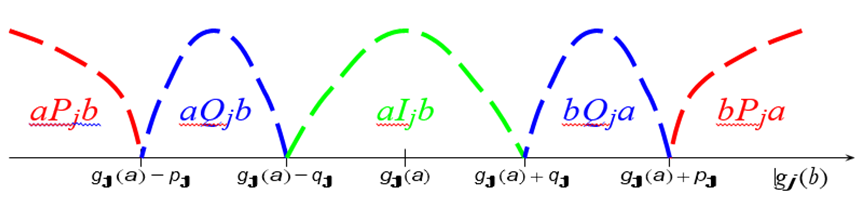
\includegraphics{aide_multicrit_decision/intervales_pref_inconp_indif.png}
\end{center}
\caption{approche de sur-classement}
\end{figure}

Cas particuliers:
\begin{itemize}
\item pj  = qj : quasi-critère,
\item qj  = 0 :	pré-critère,
\item pj  = qj  = 0 : vrai-critère.
\end{itemize}

La méthode Electre III s’appuie sur les étapes  suivantes :

Pour que aSb soit validée, il faut que les deux conditions suivantes soient vérifiées :
\begin{enumerate}
\item Condition  de concordance : une majorité de critères doit être en accord avec aSb (principe majoritaire),
\item Condition de non-discordance : aucun des critères non concordants ne doit réfuter fortement aSb (principe de respect des minorités).
\end{enumerate}
On peut mettre en œuvre ces principes de diverses manières comme on peut  imposer des niveaux d’exigence plus ou moins fort.

\paragraph{Évaluation des indices de concordance :}

la concordance partielle examine la contribution de chaque critère à la proposition aSb, il est obtenu comme suit :\\
Indice de concordance partielle cj (a, b) ∈ [0, 1], (j = 1, . . . , p) tel que :
\begin{itemize}
\item cj (a, b) = 0 ssi gj n’est pas du tout en faveur de aSb
\item cj (a, b) = 1 ssi gj est totalement en faveur de aSb
\item cj (a, b) ∈]0, 1[ ssi gj est partiellement en faveur de aSb
\end{itemize}
	ce qui peut se formuler par :
                      
\[
    c_{j}(a, b)= 
\begin{cases}
    1 ,& \text{if } g_{j}(a) \geq g_{j}(b) - q_{j}\\
    0 ,& \text{if } g_{j}(a) \leq g_{j}(b) - p_{j}\\
    \frac{p_{j} - (g_{j}(b)-g_{j}(a))}{p_{j} - q_{j}}  ,              & \text{sinon}
\end{cases}
\]

\begin{figure}[!h]
\begin{center}
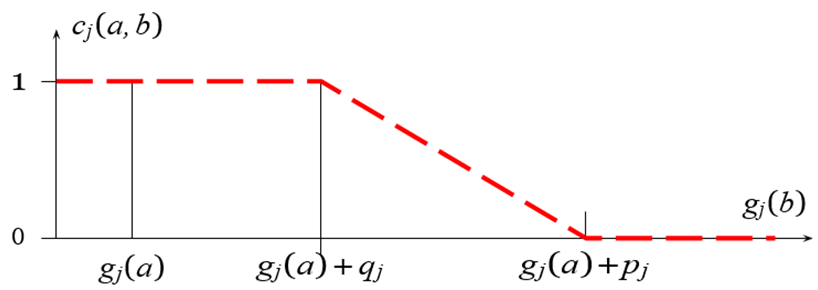
\includegraphics{aide_multicrit_decision/conc_partielle.png}
\end{center}
\caption{Concordance partielle}
\end{figure}

\paragraph{Calcul de l’indice de concordance global :}
la concordance globale apprécie la contribution de l’ensemble des critères à l’affirmation aSb
L’indice de concordance globale C(a, b) ∈ [0, 1]  tel que:
\begin{itemize}
\item C(a, b) = 0 lorsqu’aucun critère n’est en faveur de aSb
\item C(a, b) = 1 lorsque tous les critères sont en faveur de aSb
\item C(a, b) ∈]0, 1[ lorsque “certains” critères sont en faveur de aSb
\end{itemize}

Ce qui peut se formuler par :\\
\[
C(a, b) = \sum_{j=1}^{p}w_{j}c_{j}(a, b)
\]
\[\text{avec } w_{j}  \text{le poids associé au critère  } g_{j},  \sum_{j=1}^{p}w_{j} = 1\]

\paragraph{Évaluation des indices de discordance }


Parmi les critères en désaccord avec aSb, certains peuvent exprimer une forte opposition, un veto qui conduit à invalider aSb, A chaque critère gj , on associe un seuil de veto vj  tel que si gj (a) < gj (b) − vj  pour un j  donné, alors on rejette aSb (quelle que soit l’importance de la coalition concordante),  il est obtenu comme suit :

On définit, sur chaque critère, un indice de discordance partielle dj (a, b) ∈ [0, 1] tel que :
\begin{itemize}
\item dj (a, b) = 0 si gj  ne s’oppose pas à aSb
\item dj (a, b) = 1 si gj  s’oppose totalement à aSb
\item dj (a, b) ∈]0, 1[ si gj  s’oppose en partie à aSb
\end{itemize}

ce qui peut se formuler par :
\[
    d_{j}(a, b)= 
\begin{cases}
    1 ,& \text{if } g_{j}(b) - g_{j}(a) \geq  v_{j}\\
    0 ,& \text{if } g_{j}(b) - g_{j}(a) \leq  p_{j}\\
    1 - \frac{v_{j} - (g_{j}(b)-g_{j}(a))}{v_{j} - p_{j}}  ,              & \text{sinon}
\end{cases}
\]

\begin{figure}[!h]
\begin{center}
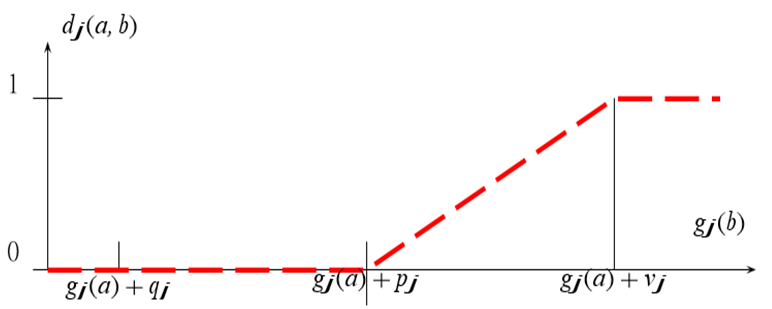
\includegraphics{aide_multicrit_decision/disc_partielle.png}
\end{center}
\caption{Discordance partielle}
\end{figure}

\paragraph{Calcul de l’indice de crédibilité et définition de la relation de sur-classement floue}
Dans Electre III, une relation de sur-classement floue est définie par l’indice de crédibilité $\sigma$(a, b) ∈ [0, 1]
\begin{itemize}
\item si aucun critère n’est discordant $\sigma$(a, b) = C(a, b)
\item si un/plusieurs critère(s) est/sont discordant(s) $\sigma$(a, b) < C(a, b)
\item si dj (a, b) = 1 pour un critère alors $\sigma$(a, b) = 0
\end{itemize}
  
ce qui peut se formuler par :

\[
\sigma(a, b) = C(a, b)\Pi_{j\in\overline{F}}\frac{1-d_{j}(a, b)}{1-C(a,b)} \in [0,1]
\]
\[\text{avec } \overline{F} = \text{\{}{j \in F  \text{ tel que } d_{j}(a, b) > C(a, b)}\text{\}}\]
\newpage
\paragraph{Comparer les indices pour avoir le classement}
On compare à la fin entre les différents indices de crédibilité $\sigma$(a, b) de chaque action et on  garde le plus grand à chaque fois c’est-à-dire on sélectionne la meilleure action et on classe les  actions de la meilleure à la moins bonne, on parle ici de distillation descendante.

\paragraph{Avantages et inconvénients}
\begin{itemize}
\item Tout d’abord, cette approche d’analyse multicritère est fondée sur une démarche constructive. En effet, le contexte dans lequel les outils multicritères sont utilisés est voué à évoluer au cours du temps et de l’information acquise.
\item Ensuite, cette méthode permet de prendre en compte les poids donnés aux critères de jugement. Cette étape de pondération permet aux différents acteurs de donner leurs opinions et d’exprimer d’éventuelles différences de jugement.
\item La simplicité de la méthode vu qu’elles reposent sur des concepts naturels, tels « d'accord » ou « pas d'accord ».
\item Enfin, ELECTRE III est une méthode multicritère fondée sur les principes de la logique floue, permettant de prendre en compte les incertitudes liées aux calculs et à l’évaluation des performances à travers l’utilisation de pseudo-critères. C’est l’une des principales caractéristiques de la méthode de pouvoir traiter, du fait de l’existence des seuils, d’évaluations dont la définition est difficile.
\item L’inconvénient avec ELECTRE est sa grande complexité et son recourt important aux valeurs numériques qui la rapprochent des méthodes d'utilité.
\end{itemize}



\section{Conclusion}
Ce chapitre présente la notion d’aide à la décision, et plus particulièrement l’aide à la décision multicritère et les deux méthodes que j’ai implémenté dans le cadre de ce travail, dans la section suivante, nous allons voir la partie conception et implémentation de l’outil d’aide à la décision pour le classement des salariés.









 
\chapter{Conception et implémentation}



\section{Introduction}

L’outil d’aide à la décision pour le classement des salariés utilise les données issues de l’application de gestion du personnel d’une entreprise afin de faire un classement de ces derniers et en déduire les employés les plus méritants d’une promotion ou prime.\\
L’outil d’aide à la décision pour le classement des salariés utilise les données issues de l’application de gestion du personnel d’une entreprise afin de faire un classement de ces derniers et en déduire les employés les plus méritants d’une promotion ou prime.\\ 

\section{Architecture éventuelle de l’application }
L’application contiendra trois onglets principaux correspondant à trois modules différents :
\begin{enumerate}
\item L’onglet gestion du temps et absence
\item L’onglet gestion de l’activité quotidienne 
\item L’onglet informations personnelles 
\end{enumerate}

\subsection{Onglet gestion du temps et absence }

Cet onglet devrait contenir toutes les informations relatives aux absences (le nombre de jours où il s’est absent, les congés payés, les congés sans solde, les ponts, les RTT, ...etc).\\

Ces informations seront insérées par le salarié avant la fin du mois et validées par son manager à la fin du mois.

\subsection{Onglet gestion de l’activité quotidienne}

Dans cette section on retrouvera les informations relatives à l’activité quotidienne du salarié c’est-à-dire les taches qui lui sont affectées, la durée estimée pour leur réalisation, la durée réellement réalisée, la difficulté de la tâche, l’évaluation du travail effectué.\\
Le chef de projet s’occupe d’affecter les taches et d’estimer la durée de leur réalisation ainsi que leur difficulté en présence du n+1 du salarié et le salarié lui-même et cela durant les différentes réunions hebdomadaires par exemple.\\
Une fois la tache effectuée, le salarié insérera la durée réelle passée sur la tâche et qui pourrait s'avérer supérieure, égale ou inférieure à la durée estimée pour cette dernière.\\
Quant à l’évaluation du travail effectué, ça sera fait par le manager ou le n+1 et par le client (s’il y en a un) et cela en présence du salarié.          

\subsection{Onglet informations personnelles}

Cet onglet concerne plus les informations relatives au salarié telles que l'identifiant du salarié, nom, prénom, âge, adresse, numéro de téléphone, … le nombre d’années au sein de l’entreprise, le rang hiérarchique, les promotions et primes obtenues avec la date de chacune, le nombre total de promotion et prime obtenues, classement obtenu à la dernière réunion d’attribution de prime ou de promotion, une note d’appréciation.\\


Le salarié ainsi que ses supérieurs auront un accès en lecture seule sur ces informations, qui en réalité seront affichées directement de la base de donnée par le système en place. \\
La note d’appréciation quant à elle est calculée chaque mois par le système en utilisant les votes anonymes des salariés de l’entreprise. Le système d’évaluation propose 5 types d’appréciation d’après le tableau suivant :    

\begin{figure}[!h]
\begin{center}
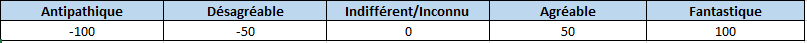
\includegraphics[height=0.8cm]{Conception_implementation/tableau_sym.png}
\end{center}
\caption{tableau notes salarié}
\end{figure}

En ce qui concerne le classement obtenu à la dernière réunion d’attribution de prime ou de promotion c’est justement le sujet principal de ce travail, j’en parlerai plus en détail dans les sections suivantes mais en générale le système calculs et retourne d’après différents critères appliqués aux salariés un classement de ces derniers du plus méritant d’une promotion (ou prime) au moins méritant, donc le classement obtenu lors de la dernière exécution du système sera affiché sur le profil du salarié .      

\section{Historisation Mensuelle}

A chaque fin de mois l’application fait une historisation des informations récoltées concernant chaque salarié de l’entreprise.  

\section{Analyse des données récoltées }

Afin de pouvoir faire un classement des salariés notre système a besoin d’un fichier Excel ou d’une Base de données directement en entrée.\\
Ce fichier Excel contiendra l’ensemble des actions, critères et poids dont le système a besoin pour effectuer le classement des salariés. Pour construire ce fichier, nous nous proposons d'utiliser l'ETL qui va effectuer une collecte de données à partir d’un magasin de données dédié à cet effet et récolter les mesures (indicateurs) qui nous intéressent sur les salariés et ce sous format Excel. \\
Le magasin de données sera construit toujours grâce à l’ETL durant la phase d’alimentation qui se fera à partir de la base de données de production. Et, c’est durant cette phase là que le calcul des indicateurs « mesures » se fera grâce aux requêtes analytiques.  \\
\newpage
Les indicateurs « mesures » choisi pour ce travail sont les suivants:
\begin{enumerate}
\item Les compétences et Les résultats (productivité de l’employé)   I1
\item Les appréciations sociales  I2
\item La pénibilité du travail   I3
\item L’ancienneté dans l'entreprise   I4
\item L’assiduité (Les présences et les absences)    I5
\end{enumerate}

\subsection{Compétences et Les résultats (productivité de l’employé)}
Cet indicateur est calculé à partir de l’évaluation du travail effectué et temps passé sur la tâche, et faire une moyenne des deux critères. \\
Le score obtenu pour l’évaluation du travail effectué est récupéré directement de la base de données et sa valeur est répartie entre 0 et 100. Quant au score obtenu pour le temps passé sur la tâche, il est déduit à partir de la règle suivante :\\

On part du principe que si un travail est effectué en temps voulu c’est-à-dire « durée estimée = durée réelle effectuée » alors le salarié obtient un score de 50\%. Et à partir de cette base là ,on calcule les autres scores, et pour exemple : un salarié ayant effectué une tache dont la durée était estimée à 5 jours en seulement  3 jours  aurait un score de 70\%.\\

Pour finir, on calculera la moyenne de ces scores sur tous les mois compris dans l’évaluation semestrielle ou annuelle.  La récupération de ces scores est possible grâce à l’historisation mensuelle.  


\subsection{Appréciations sociales}
Pour cet indicateur, on n'a pas besoin de calcul car on a déjà le score dans le format voulu grâce à l’application de vote anonyme dont les valeurs varient entre -100 et 100.   \\
Ensuite, on calculera la moyenne de ces scores sur tous les mois compris dans l’évaluation semestrielle ou annuelle, étant donné que le vote se fait de manière mensuelle. La récupération de ces informations est possible grâce à l’historisation mensuelle.

\subsection{Pénibilité du travail}
Comme pour l’indicateur précédent et comme expliqué plus haut, le score est déjà calculé et saisis par le chef de projet manuellement avec une notation entre 1 et 100.\\
Ensuite, on calculera la moyenne de ces scores sur tous les mois compris dans l’évaluation semestrielle ou annuelle et cela grâce à l’historisation mensuelle. 


\subsection{Ancienneté dans l'entreprise }
 Cet indicateur est calculé d’après le nombre d’années passées dans l’entreprise, à savoir directement le nombre d’années compris entre 0 et 40 ans.\\
Cet indicateur est mis à jour chaque année. 


\subsection{Assiduité « les présences et les absences »}
Le calcul de cet indicateur se fera mensuellement suivant le principe utilisé pour le calcul du premier indicateur « I1 », c’est-à-dire qu'on considère pour une personne qui a 0 absence durant le mois équivaut à 100\%, et à partir de cette règle, on en déduira les autres.\\
Ensuite, on calculera la moyenne de ces scores sur tous les mois compris dans l’évaluation semestrielle ou annuelle grâce à l’historisation mensuelle. 


\section{Classement des salariés }
L’outil d’aide à la décision pour le classement des salariés, Prend en entrée un fichier Excel « que je suppose déjà crée » contenant la matrice de performance et retourne un classement des salariés sur un autre fichier Excel.\\ 
Pour effectuer cela, j’ai choisis de tester deux méthode d’analyse multicritère LA SOMME PONDÉRÉE et ELECTRE III.\\

Le premier et deuxième point de ce qui suit concernent les démarches communes effectuées pour les deux méthodes

\begin{enumerate}
\item Détermination des critères :
\\
J’ai choisis 5 critères pertinents après avoir questionné quelques Managers.
      \begin{itemize}
      \item Les compétences et Les résultats (productivité de l’employé)
      \item Les appréciations sociales
      \item La pénibilité du travail
      \item L’ancienneté dans l'entreprise
      \item Les présences et les absences     
      \end{itemize}
      
\begin{figure}[!h]
\begin{center}
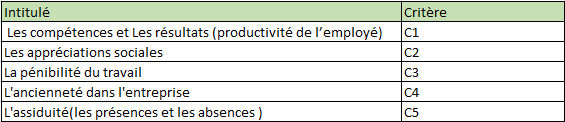
\includegraphics{Conception_implementation/noms_criteres.png}
\end{center}
\caption{Le tableau des critères retenus}
\end{figure}

\newpage

\item Pondération des critères :
\\
Le premier et deuxième point de ce qui suit concernent les démarches communes effectuées pour les deux méthodes

\begin{figure}[!h]
\begin{center}
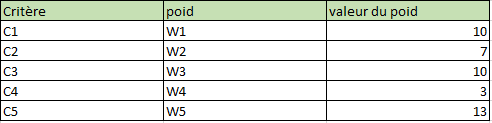
\includegraphics{Conception_implementation/poids.png}
\end{center}
\caption{Le tableau de pondération des critères 1}
\end{figure}


Le tableau des poids utilisé en entré du programme :
\begin{figure}[!h]
\begin{center}
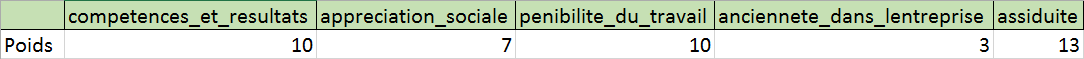
\includegraphics[width=16cm]{Conception_implementation/poids_en_entr_s.png}
\end{center}
\caption{Le tableau de pondération des critères 2}
\end{figure}


\item Détermination des seuils :
\\
J’ai choisi de donner la même valeur de seuil de préférence et de seuil d’indifférence a tous les critères Pj = Qj = 0 pour avoir le cas particulier de vrai critère et éviter le cas d’incomparabilité « aQb » et d’indifférence « aIb » entre deux action.

\begin{figure}[!h]
\begin{center}
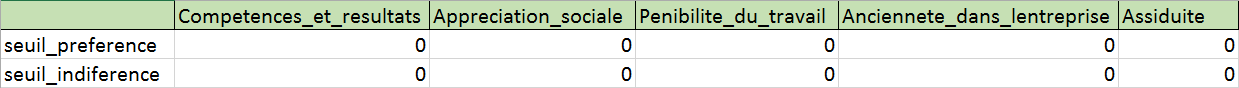
\includegraphics[width=16cm]{Conception_implementation/seuils.png}
\end{center}
\caption{Le tableau des seuils de préférences et d’indifférences attribués aux critères}
\end{figure}

Pour le veto, les valeurs sont différentes d’après l’importance du critère. Sur certains l’effet de veto est supprimé, considérant de façon arbitraire que la nature de ces critères n’amène pas forcément à refuser le sur-classement d’une action sur l’autre si la différence de leur performance dépasse une certaine valeur.    

\begin{figure}[!h]
\begin{center}
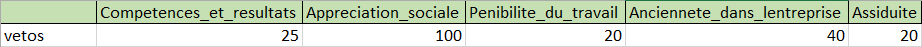
\includegraphics{Conception_implementation/veto.png}
\end{center}
\caption{Le tableau des seuils de préférences et d’indifférences attribués aux critères}
\end{figure}

\end{enumerate}

\newpage


\section{Implémentation}

 Pour effectuer le classement des salariés, on avait choisi de tester deux méthodes d’analyses multicritère à savoir la somme pondérée et ELECTRE III, que j’ai implémenté avec le langage python.


\subsection{ELECTRE }
\subsubsection{Évaluation des indices de concordance :}
La fonction qui permets de vérifier la concordance partielle :
\begin{lstlisting}[language=Python, frame=single, firstnumber=127]
def concord_parti(gs1, gs2, critere):
    if gs1 >= gs2 - seuil_indiference[critere]:  
        return 1
    elif gs1 <= gs2 - seuil_preference[critere]:  
        return 0
    else:
        return (seuil_preference[critere] - (gs2 - gs1)) / (seuil_preference[critere] - seuil_indiference[critere])
\end{lstlisting}

\subsubsection{Calcul de l’indice de la concordance globale :}
La fonction qui permets de calculer l’indice de la concordance globale :

\begin{lstlisting}[language=Python, frame=single, firstnumber=137]
def concord(s1, s2):
    conc = 0.0
    for critere in Criteres:
        poids = Poids[critere]
        
        gs1 = Performances[s1][critere]
        gs2 = Performances[s2][critere]
        c = concord_parti(gs1, gs2, critere)
        conc += c * poids
        
    print("    concordance entre : "+s1+" et "+s2+" est : "+str(conc) )
    return conc  
\end{lstlisting}

\subsubsection{Évaluation des indices de discordance partielle:}
\begin{lstlisting}[language=Python, frame=single, firstnumber=90]
def discord_parti(gs1, gs2, veto, critere):
    diff = gs2-gs1
    if (gs1 < 0) & (gs2 < 0) :
        diff = abs(gs2 - gs1)
        
    if diff >= veto:
        return 1
    elif diff <= seuil_preference[critere]:
        return 0
    else :
        res = 1 - ((veto - diff)/(veto - seuil_preference[critere]))
        return res
\end{lstlisting}

\newpage

\subsubsection{Évaluation des indices de discordance globale:}
\begin{lstlisting}[language=Python, frame=single, firstnumber=106]
def discord(s1, s2, conc):
    app_disc = appliquer_disc(s1, s2, conc)
    disc = 1.0
    if app_disc == True:
        for critere in Criteres:
            veto = vetos[critere]
            gs1 = Performances[s1][critere]
            gs2 = Performances[s2][critere]
            d = discord_parti(gs1, gs2, veto, critere)
            if d > conc :
                tmp = (1-d)/(1-conc)
                disc *=  tmp
                   
        print("        discordance entre : "+s1+" et "+s2+" est : "+str(disc) )
    return disc
\end{lstlisting}

\subsubsection{Calcul de l’indice de crédibilité :}
\begin{lstlisting}[language=Python, frame=single, firstnumber=157]
def credibilite(ks1, ks2):
    conc = concord(ks1, ks2)
    disc = discord(ks1, ks2, conc)
    cred = conc * disc
    return cred
\end{lstlisting}


\subsubsection{Le classement des salariés}
\begin{lstlisting}[language=Python, frame=single, firstnumber=157]
# retourne meilleur entre 2 salaries
def compare_2_salarie(ks1, vs1, ks2, vs2):
    print("Calcule credibilite entre "+ks1+" et "+ks2+" et l'inverse : ")
    cred1 = credibilite(ks1, ks2)
    cred2 = credibilite(ks2, ks1)
    print("credibilite "+ks1+" et "+ks2+" : "+str(cred1))
    print("credibilite "+ks2+" et "+ks1+" : "+str(cred2))
    if cred1 >= cred2:
        print("*********** "+ks1+" surclasse "+ks2+" *********** ")
        return ks1, vs1
    else :
        print("*********** "+ks2+" surclasse "+ks1+" *********** ")
        return ks2, vs2
\end{lstlisting}
\newpage
\subsection{Somme pondéré }
\subsubsection{Normalisation des données }
Cette fonction permet à partir de la matrice de décision (le tableau des performances) d’aboutir à une matrice normalisée, j’ai choisis la procédure de normalisation suivante  : \\
n étant le nombre de critères, on a:
\begin{align*}
v_{i} = \frac{a_{i}}{\sum_{i=1}^{n}a_{i} }, \forall i \in [1, m]
\end{align*}
\begin{lstlisting}[language=Python, frame=single, firstnumber=63]
def normalisation_data(performances):
    print("\n\n")
    print("************************ donnees normalisees ************************")
    for p in performances.keys():
        somme_ligne = sum(performances[p].values())
        for c in performances[p].keys():
            performances[p][c] = performances[p][c]/somme_ligne
        
    print_data(performances)
    print("\n\n\n\n")                      

\end{lstlisting}

\subsubsection{Normalisation du poids de chaque critère}
Cette fonction permets de normaliser le vecteur des poids toujours en appliquant la procédure :\\
n étant le nombre de critères, on a:
\begin{align*}
v_{i} = \frac{w_{i}}{\sum_{i=1}^{n}w_{i}}, \forall i \in [1, m]
\end{align*}

\begin{lstlisting}[language=Python, frame=single, firstnumber=49]
weights = dict(zip(crit, map(lambda p: p/sum(weights), weights)))
\end{lstlisting}

\subsubsection{Mise en œuvre de la méthode somme pondérée :}
Cette fonction permets d’appliquer la procédure : \\
n étant le nombre de critères et m le nombre de salariés
\begin{align*}
R(a_{i}) = \sum_{j=1}^{n}w_{j}a_{ij}, \forall i \in [1, m]
\end{align*}

si on prend la première ligne pour exemple on a le calcul suivant :
\begin{align*}
R(a_{1}) = w_{1}a_{11}+w_{2}a_{12}+w_{3}a_{13}+w_{4}a_{14}+w_{5}a_{15}
\end{align*}

\begin{lstlisting}[language=Python, frame=single, firstnumber=76]
def somme_pond(s):
    sp = 0.0
    for critere in Criteres:
        poids = Poids[critere]
        gs = Performances[s][critere]
        sp += (gs * poids)
        
    return s, sp
\end{lstlisting}

\section{Conclusion}
Ce chapitre présente la conception de l’outil d’aide à la décision pour le classement des salariés « le principe de récupération des données utilisées pour le classement, les méthodes d’analyses multicritères sélectionnées pour le classement » mais surtout l’implémentation détaillée des différentes fonctions utilisées pour le classement des salariés dans le cas des deux méthodes d’analyse multicritères à savoir la Somme pondérée et ELECTRE III.\\
Les résultats obtenus par ces deux méthodes seront détaillés dans le chapitre suivant. 


%\chapter{Autre partie}

Dans cette partie nous cherchons à décrire dans un premier temps [...], puis, c[...].

\section{Partie 1}

Intro

\subsection{Sous-partie 1}

\begin{figure}[!ht]
\begin{center}

\includegraphics[height=12cm]{autre_partie/image1}
\end{center}
\caption[autre partie générale]{autre partie image 1\protect\footnotemark}
%\floatfoot{Source: (Citation command)}
% avec le package "floatrow"
\end{figure}

%footnote protected pour apparaitre dans la légende d'une image
\footnotetext{Schéma d'après : \textit{Auteur 1 \& Propriétaire image}, LICENCE (cf. ref. \cite{cite4})}

\newpage{}

\subsection{Sous-partie 2}

\begin{figure}[!ht]
\begin{center}

\includegraphics[height=12cm]{autre_partie/image2}
\end{center}
\caption[autre partie]{autre partie globale de notre quelque chose}
\end{figure}

Nous retrouvons ici, blabla\footnote{Application bla - Interface blabla} [...].

\subsubsection{Sous-sous-partie 1}

Le bla (cf. ref. \cite{cite6}) est [...]:

\begin{itemize}
\item item1;
\item item2;
\item item3;
\item item4;
\item item5.
\end{itemize}

\newpage

\subsubsection{Sous-sous-partie 2}

%Les lignes :
% \setcounter{secnumdepth}{4}
% \setcounter{tocdepth}{4}
%dans le fichier "main.tex" permettent de faire en sorte que les paragraphes soient interprété comme des titres de niveau 5
\paragraph{Paragraphe 1 (agissant comme titre niveau 5)}
%forcer un saut de ligne
~\\
\hskip7mm

\begin{figure}[!ht]
\begin{center}

\includegraphics[height=6cm]{autre_partie/image3}
\end{center}
\caption[Structure d'unz autre chose]{Structure d'une autre chose\protect\footnotemark}
\end{figure}

Ce schéma représente bla.

\footnotetext{Schéma et explication d'après le wiki bla (cf. ref. \cite{cite0})}

\paragraph{Paragraphe 2}
~\\
\hskip7mm

%fixer les floats précédemment définis
%\FloatBarrier

Bla

\subparagraph{Sous-paragraphe 1}
~\\
\hskip7mm

Bla

\begin{figure}[H]
\begin{center}

\includegraphics[height=10cm]{autre_partie/image4}
\end{center}
\caption{Diagramme de truc}
\end{figure}

\subparagraph{Sous-paragraphe 2}
~\\
\hskip7mm

Bla\\

Bla

\subparagraph{Sous-paragraphe 3}
~\\
\hskip7mm

Bla

\subsubsection{Sous-sous-partie 3}

Bla

\section{Partie 2}

Bla

\footnotetext{D'après le schéma disponible sur la documentfation officielle disponible sur le site blalbla}

Bla

\subsection{Sous-partie 1}

Bla

\subsection{Sous-partie 2}

Bla

\paragraph*{Paragraphe 1 (n'apparaitra pas dans l'index)}
Bla

\paragraph*{Paragraphe 2}
Bla

\paragraph*{Paragraphe 3}
Bla

\subsection{Sous-partie 3}

Bla

\chapter{Résultats}

\section{Introduction}
Afin d’avoir un jeu de données assez riche, varié et aussi complet que possible et surtout réaliste, j’ai dû passer par plusieurs entreprises, essuyer plusieurs refus en raison de la confidentialité et de la protection des informations des salariés, pour parvenir à me procurer une liste anonyme d’une dizaine de salariés qui me servira de base de travail.

\section{Le jeu de données pour le test :}
Ce sont les résultats des salariés de l’entreprise du semestre passé qui m'ont permis d'élaborer la matrice de décision sous forme du « tableau des performances » ci-dessous : 

\begin{figure}[!h]
\begin{center}
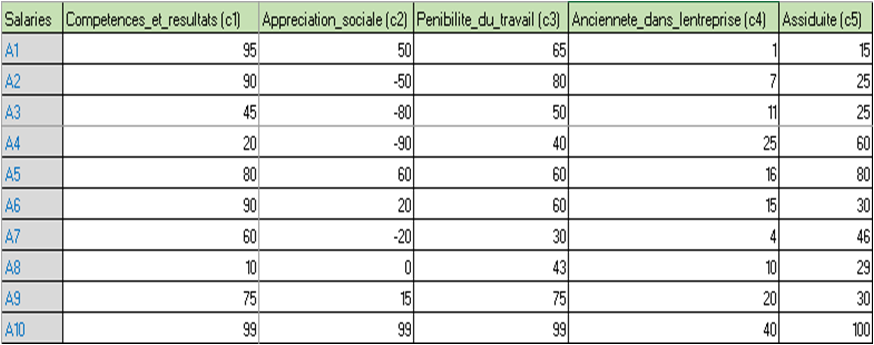
\includegraphics{Tests_resultats/performances_salaries.png}
\end{center}
\caption{tableau des performances des salariés}
\end{figure}

\section{Les résultats :}
Pour vérifier les résultats de mon programme sur cette matrice, j’ai comparé mes résultats obtenus avec l’application des deux méthodes «la méthode de la somme pondérée et la méthode ELECTRE III » avec le cas réel, c’est-à-dire les salariés qui ont réellement reçu une promotion à la fin du semestre dernier au sein de l’entreprise.
\newpage

\begin{itemize}
\item Le classement des salariés d’après l’entreprise :
\begin{figure}[!h]
\begin{center}
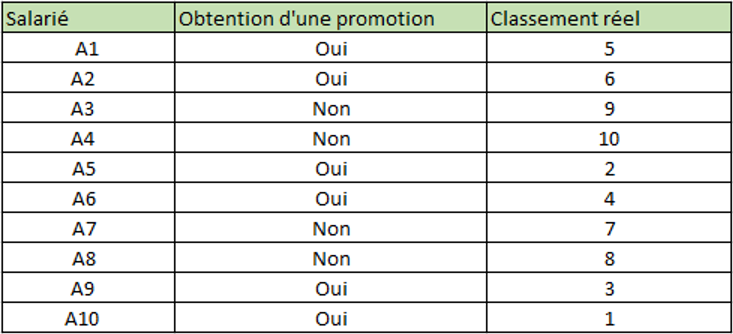
\includegraphics{Tests_resultats/classement_salarie.png}
\end{center}
\caption{classement des salariés d’après l’entreprise}
\end{figure}

\item Le classement des salariés avec la méthode de la somme pondérée
\begin{figure}[!h]
\begin{center}
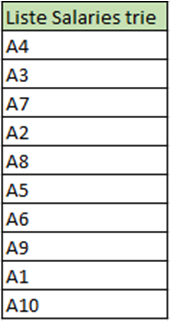
\includegraphics{Tests_resultats/classement_somme_pondere.png}
\end{center}
\caption{résultat du classement des salariés avec la méthode de la somme pondérée}
\end{figure}

\item Le classement des salariés avec la méthode ELECTRE III
\begin{figure}[!h]
\begin{center}
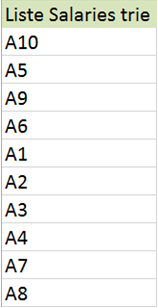
\includegraphics{Tests_resultats/classement_electre.png}
\end{center}
\caption{résultat du classement des salariés avec la méthode ELECTRE III}
\end{figure}

\section{Explication des résultats :}
D’après les résultats obtenus, on remarque clairement que le résultat affiché avec la méthode ELECTRE se rapproche de manière considérable du classement réel des salariés de l’entreprise, contrairement au résultat obtenu avec la méthode de la somme pondérée qui, elle, affiche un résultat diffèrent.\\
Ces résultats s’expliquent du fait que la méthode ELECTRE est plus adaptée pour les analyses d’aide à la décision multicritère où on a de nombreux critères qui entrent en jeu. Quant à la méthode de la somme pondérée ses résultats sont plus efficaces quand on considère un seul critère par exemple « si le salarié a atteint ou pas son objectif » ce qui est fait dans la méthode MBO. 


\section{Conclusion :}
Dans ce chapitre on a présenté tout d’abord, les tests effectués ainsi que les résultats obtenus suite à l’application des deux méthodes d’analyses multicritères « la Somme pondérée et ELECTRE III » sur les données de performances des salariés. Puis, on a effectué une comparaison des résultats obtenus. Dans le chapitre suivant seront développées les perspectives ainsi que la conclusion.
\end{itemize}


\chapter*{Conclusion}
\addcontentsline{toc}{chapter}{Conclusion}


La problématique de décision multicritère est souvent présente dans la vie pratique. Du simple choix d’un achat à la sélection d’une carrière, la question demeure la même : comment faire le bon choix en tenant compte de toutes les contradictions qui existent dans les critères qui participent au processus de décision ? La problématique de décision multicritère se réfère à une prise de décision en présence de plusieurs critères, souvent contradictoires.
\vspace{5mm}

Pour les entreprises, une des décisions la plus importante et critique à prendre consiste dans le choix des salariés les plus méritants d’une promotion ou prime et dont le choix doit se faire de manière juste et équitable pour éviter tout sentiment de mise à l’écart de certains salariés ou de favoritisme pour d’autres. Pour aider à cette prise de décision, une solution possible serait de les classer par ordre du plus méritant au moins méritant et cela en les évaluant sur 5 critères majoritairement jugés importants par les entreprises à savoir « les compétences et les résultats, les appréciations sociales, la pénibilité du travail, l’ancienneté dans l’entreprise, l’assiduité», Pour avoir ce classement, on utilise les méthodes d’analyse multicritère « Somme pondérée, ELECTRE III … » des méthodes qui ont déjà montrées leurs efficacités dans de nombreux domaines. Cependant, il est difficile d’estimer les paramètres de ces méthodes qui, utilisent des poids pour quantifier l’importance de chaque critère dans le processus de décision. De ce fait, quand les alternatives offertes par la méthode ne sont pas conformes aux préférences du décideur, une interaction entre la méthode et ce dernier est indispensable afin d’affiner le processus de décision et par conséquent  le processus n’est pas à 100\% automatisé. Une alternative possible à cela « perspective » serait d’utiliser « Les systèmes autonomes dynamiques», qui sont des systèmes auto adaptatifs, capables d’apprendre le comportement de leur environnement afin de s’auto-configurer et de prendre des décisions optimales, sans avoir recours à une aide externe.



%%Ne pas numéroter cette partie
\part*{Annexes}
%Rajouter la ligne "Annexes" dans le sommaire
\addcontentsline{toc}{part}{Annexes}

\chapter*{Annexe 1}
\addcontentsline{toc}{chapter}{Annexe 1}

%changer le format des sections, subsections pour apparaittre sans le num de chapitre
\makeatletter
\renewcommand{\thesection}{\@arabic\c@section}
\makeatother

%recommencer la numérotation des section à "1"
\setcounter{section}{0}

Intro

\section{Partie 1}

Bla

\subsection{Sous-partie 1}

Bla

\subsection{Sous-partie 2}

Bla

\subsection{Sous-partie 3}

Bla

\section{Partie 2}

Bla

\subsection{Sous-partie 1}

Bla

\subsection{Sous-partie 2}

Bla

\subsection{Sous-partie 3}

Bla

\chapter*{Annexe 2}
\addcontentsline{toc}{chapter}{Annexe 2}

%recommencer la numérotation des section à "1"
\setcounter{section}{0}

Intro

\section*{Prérequis}
\addcontentsline{toc}{section}{Prérequis}

Bla

\begin{itemize}
\item item1;
\item item2;
\item item3;
\item item4.
\end{itemize}

Bla

\section{Partie 1}

Bla

\subsection{Sous-parie 1}

Bla

\subsection{Sous-parie 2}

Bla

\section{Partie 2}

\begin{center}
\textsc{Attention !}

\textit{Texte d'avertissement}
\end{center}

Bla

\newpage

\section{Partie 3}

Bla

\begin{figure}[!ht]
\begin{center}
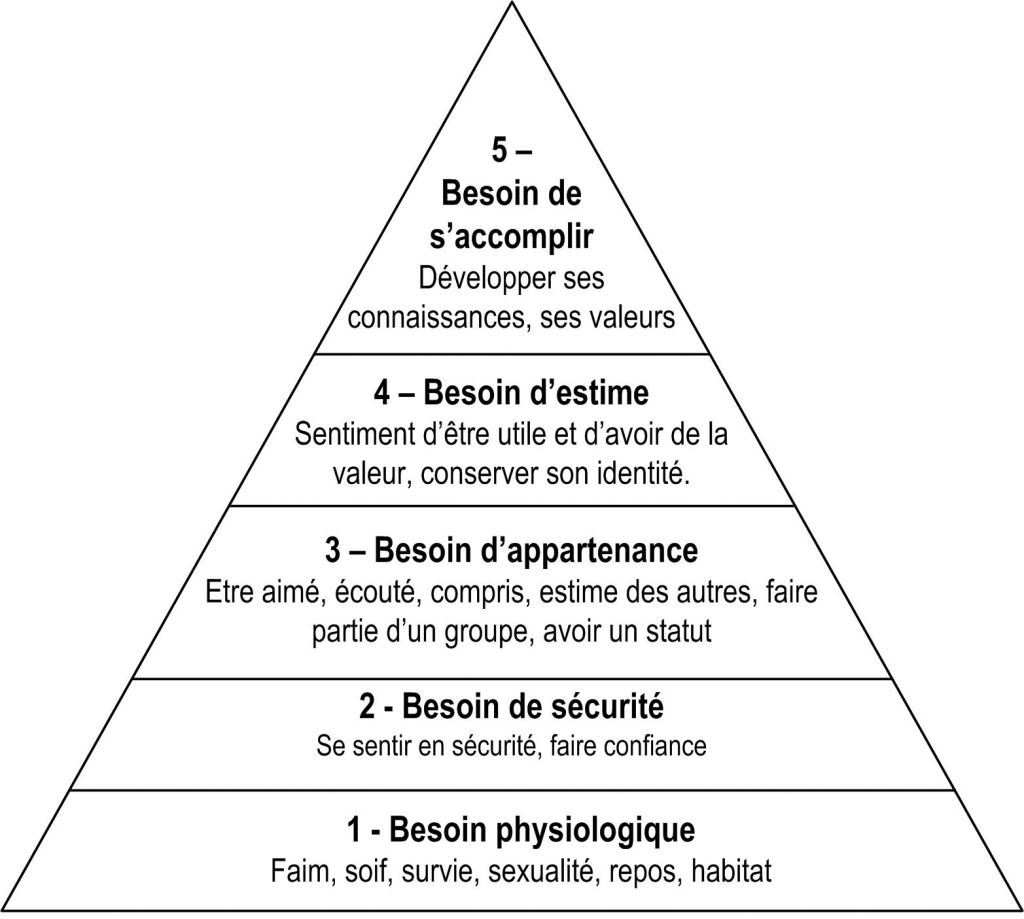
\includegraphics[height=8cm]{introduction/schema_introduction}
\end{center}
\caption[schema]{Presentation schema}
\end{figure}

\paragraph*{Paragraphe 1}
~\\
\hskip7mm

Bla

\paragraph*{Paragraphe 2}
~\\
\hskip7mm

Bla

\paragraph*{Paragraphe 3}
~\\
\hskip7mm

Bla

\newpage

%récupérer les citation avec "/footnotemark"
\nocite{*}

%choix du style de la biblio
\bibliographystyle{plain}
%inclusion de la biblio
\bibliography{bibliographie.bib}
%voir wiki pour plus d'information sur la syntaxe des entrées d'une bibliographie

\end{document}